
\documentclass[brazil]{beamer}

\usepackage[utf8]{inputenc}
\usepackage{babel}

\usepackage{pgfpages}

\setbeameroption{show notes on second screen=right}

\usetheme[
    titleformat=allcaps,
    progressbar=foot,
    block=fill]{metropolis}           % Use metropolis theme

\usepackage{tikz}
    \usetikzlibrary{shapes.symbols, shapes.callouts, arrows, calc, backgrounds, fit}
    
    \makeatletter
    \newcommand{\gettikzxy}[3]{%
      \tikz@scan@one@point\pgfutil@firstofone#1\relax
      \edef#2{\the\pgf@x}%
      \edef#3{\the\pgf@y}%
    }
    \makeatother

    \tikzstyle{arrow} = [thick,->,>=stealth]

\usepackage{subfigure}
\usepackage{graphicx}

\usepackage{hyperref}
\usepackage{textcomp}

%% Para estilizar emails
\catcode`\_=11\relax
\newcommand\email[1]{\_email #1\q_nil}
\def\_email#1@#2\q_nil{%
    \textlangle{}\href{mailto:#1@#2}{{\emailfont\detokenize{#1}\emailampersat\detokenize{#2}}}\textrangle{}%
}
\newcommand\emailfont{\ttfamily}
\newcommand\emailampersat{{\color{red}\small@}}
\catcode`\_=8\relax
%% --

\usepackage[autostyle,portuguese=brazilian]{csquotes}

    \def\signed #1{{\leavevmode\unskip\nobreak\hfil\penalty50\hskip1em
    \hbox{}\nobreak\hfill #1%
    \parfillskip=0pt \finalhyphendemerits=0 \endgraf}}

    \newsavebox\mybox
    \newenvironment{aquote}[1]
    {\savebox\mybox{#1}\begin{quote}\openautoquote\hspace*{-.7ex}}
    {\unskip\closeautoquote\vspace*{1mm}\signed{\usebox\mybox}\end{quote}}

\usepackage{transparent}

\title{Estruturas de Dados \\ e Viagem no tempo}
\date{\vspace*{1.5em} \large V SESCOMP --- 2019}
\author{{{\Large Arthur Araruna}\raisebox{1ex}{$\alpha$}} \\ \scriptsize \email{ararunaufc@gmail.com}}
\institute{\vspace*{3em} \scriptsize \raisebox{1ex}{$\alpha$}Universidade Federal do Ceará \\ \hphantom{\raisebox{1ex}{$\alpha$}}Campus de Quixadá}

\begin{document}
    \logo{
\includegraphics[height=.8cm]{../../ufc-qxd-hor-col.png} \hspace*{.3cm}}
    \frame{\titlepage}


    \logo{\transparent{0.4}
\includegraphics[height=.8cm]{../../ufc-qxd-hor-col.png} \hspace*{.3cm}}
    \begin{frame}
        \frametitle{Ressalvas}

    \end{frame}

\section{Viagem no Tempo (segundo a física)}

\section{Viagem no Tempo (segundo a ficção)}

\section{Estruturas de Dados Temporais}

    \begin{frame}
        \frametitle{Terminologia}

        \begin{itemize}
            \item Consultas {\em vs.} Atualizações
            \note[item]{{\em Operações:} Todas as operações que podemos realizar numa estrutura realizam alguma tarefa que pode ser classificada entre \underline{obter uma informação} (obter a resposta a uma pergunta) ou \underline{realizar uma alteração na organização}.}
            \note[item]{{\em Operações:} Existem certas operações que podem se comportar de ambas as formas, mas sempre podemos subdividí-las.}
            \item Versão
            \note[item]{{\em Versão:} Cada configuração (ou estado) de uma estrutura de dados após uma operação de Atualização.}
        \end{itemize}
    \end{frame}

    \begin{frame}
        \frametitle{Estruturas de Dados Temporais}

        \begin{itemize}
            \item Efêmeras
            \begin{itemize}[<2->]
                \item Apenas uma versão (a última) está disponível para manipulação.
                \note[item]{{\em Efêmeras:} As estruturas que chamamos de ``Estruturas de Dados''.}
                \note[item]{{\em Efêmeras:} Efêmero significa passageiro, que dura pouco. Qualquer estado da estrutura dura apenas até a próxima atualização.}
                \note[item]{{\em Efêmeras:} Modelo de memória de um computador. Uma vez feito, não se sabe o que estava lá antes.}
            \end{itemize}
            \item Persistentes
            \begin{itemize}[<3->]
                \item Todas as versões da estrutura estão disponíveis (com ressalvas) para manipulação.
                \item Atualizações em alguma versão {\em não se propagam} para as demais.
                \note[item]{{\em Persistentes:} Se comportam em analogia à visão que a física tem sobre viagem no tempo.}
            \end{itemize}
            \item Retroativas
            \begin{itemize}[<4->]
                \item Todas as versões da estrutura estão disponíveis (com ressalvas) para manipulação.
                \item Atualizações em alguma versão {\em sempre se propagam} para as demais.
                \note[item]{{\em Retroativas:} Se comportam em analogia à visão que algumas obras de ficção tem sobre viagem no tempo.}
            \end{itemize}
        \end{itemize}
    \end{frame}

\section{Um último enredo a analisar}

    {
    \usebackgroundtemplate{\transparent{0.4}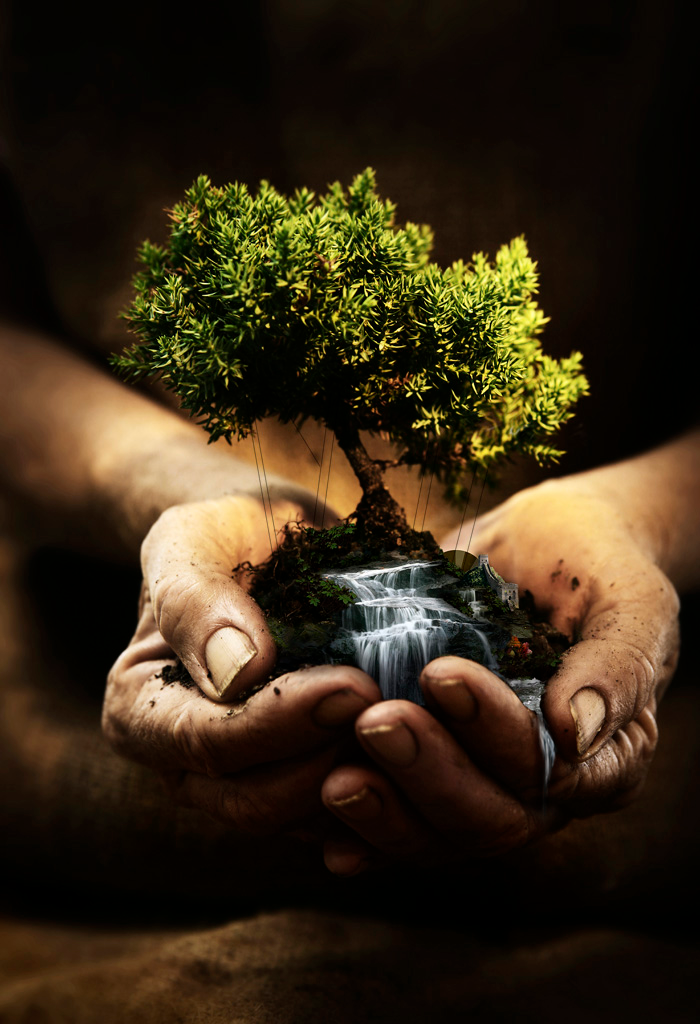
\includegraphics[height=\paperheight]{img/save_the_nature.png}}
    \begin{frame}

        \setbeamercolor{item}{fg=black}
        \setbeamercolor{normal text}{fg=black}
        \usebeamercolor[fg]{normal text}
        \begin{aquote}{???~\cite{abcd}}
            Imagine um mundo onde viagem no tempo não exista, nem seja possível. Onde suas ações são imutáveis e você só tenha uma chance. E onde não existam reviravoltas para salvar o dia no final. {\bfseries O que você faria?}
        \end{aquote}
    \end{frame}
    }

    \begin{frame}[allowframebreaks]
        \frametitle{Referências}

        \begin{thebibliography}{99}
            \bibitem{abcd} (tradução livre). Disponível em \url{www.youtube.com}.
        \end{thebibliography}
    \end{frame}
\end{document}